
\documentclass[letterpaper,hide notes,xcolor={table,svgnames},pdftex,10pt]{beamer}
\def\showexamples{t}


%\usepackage[svgnames]{xcolor}

%% Demo talk
%\documentclass[letterpaper,notes=show]{beamer}

\usecolortheme{crane}
\setbeamertemplate{navigation symbols}{}

\usetheme{PlamPittsburgh}
%\usetheme{Frankfurt}

%\usepackage{tipa}

\usepackage{textcomp}
\usepackage{hyperref}
\usepackage{graphicx,xspace}
\usepackage[normalem]{ulem}
\usepackage{multicol}
\usepackage{amsmath,amssymb,amsthm,graphicx,xspace}
\newcommand\SF[1]{$\bigstar$\footnote{SF: #1}}

\usepackage[default]{sourcesanspro}
\usepackage[T1]{fontenc}
\usepackage[scaled]{beramono}
\usepackage{tikzpagenodes}

\newcounter{tmpnumSlide}
\newcounter{tmpnumNote}


% old question code
%\newcommand\question[1]{{$\bigstar$ \small \onlySlide{2}{#1}}}
% \newcommand\nquestion[1]{\ifdefined \presentationonly \textcircled{?} \fi \note{\par{\Large \textbf{?}} #1}}
% \newcommand\nanswer[1]{\note{\par{\Large \textbf{A}} #1}}


 \newcommand\mnote[1]{%
   \addtocounter{tmpnumSlide}{1}
   \ifdefined\showcues {~\tiny\fbox{\arabic{tmpnumSlide}}}\fi
   \note{\setlength{\parskip}{1ex}\addtocounter{tmpnumNote}{1}\textbf{\Large \arabic{tmpnumNote}:} {#1\par}}}

\newcommand\mmnote[1]{\note{\setlength{\parskip}{1ex}#1\par}}

%\newcommand\mnote[2][]{\ifdefined\handoutwithnotes {~\tiny\fbox{#1}}\fi
% \note{\setlength{\parskip}{1ex}\textbf{\Large #1:} #2\par}}

%\newcommand\mnote[2][]{{\tiny\fbox{#1}} \note{\setlength{\parskip}{1ex}\textbf{\Large #1:} #2\par}}

\newcommand\mquestion[2]{{~\color{red}\fbox{?}}\note{\setlength{\parskip}{1ex}\par{\Large \textbf{?}} #1} \note{\setlength{\parskip}{1ex}\par{\Large \textbf{A}} #2\par}\ifdefined \presentationonly \pause \fi}

\newcommand\blackboard[1]{%
\ifdefined   \showblackboard
  {#1}
  \else {\begin{center} \fbox{\colorbox{blue!30}{%
         \begin{minipage}{.95\linewidth}%
           \hspace{\stretch{1}} Some space intentionally left blank; done at the blackboard.%
         \end{minipage}}}\end{center}}%
         \fi%
}



%\newcommand\q{\tikz \node[thick,color=black,shape=circle]{?};}
%\newcommand\q{\ifdefined \presentationonly \textcircled{?} \fi}

\usepackage{listings}
\lstset{basicstyle=\footnotesize\ttfamily,
	breaklines=true,
	aboveskip=15pt,
  	belowskip=15pt,
	frame=lines,
	numbers=left, basicstyle=\scriptsize, numberstyle=\tiny, stepnumber=0, numbersep=2pt
}

\usepackage{siunitx}
\newcommand\sius[1]{\num[group-separator = {,}]{#1}\si{\micro\second}}
\newcommand\sims[1]{\num[group-separator = {,}]{#1}\si{\milli\second}}
\newcommand\sins[1]{\num[group-separator = {,}]{#1}\si{\nano\second}}
\sisetup{group-separator = {,}, group-digits = true}

%% -------------------- tikz --------------------
\usepackage{tikz}
\usetikzlibrary{positioning}
\usetikzlibrary{arrows,backgrounds,automata,decorations.shapes,decorations.pathmorphing,decorations.markings,decorations.text}

\tikzstyle{place}=[circle,draw=blue!50,fill=blue!20,thick, inner sep=0pt,minimum size=6mm]
\tikzstyle{transition}=[rectangle,draw=black!50,fill=black!20,thick, inner sep=0pt,minimum size=4mm]

\tikzstyle{block}=[rectangle,draw=black, thick, inner sep=5pt]
\tikzstyle{bullet}=[circle,draw=black, fill=black, thin, inner sep=2pt]

\tikzstyle{pre}=[<-,shorten <=1pt,>=stealth',semithick]
\tikzstyle{post}=[->,shorten >=1pt,>=stealth',semithick]
\tikzstyle{bi}=[<->,shorten >=1pt,shorten <=1pt, >=stealth',semithick]

\tikzstyle{mut}=[-,>=stealth',semithick]

\tikzstyle{treereset}=[dashed,->, shorten >=1pt,>=stealth',thin]

\usepackage{ifmtarg}
\usepackage{xifthen}
\makeatletter
% new counter to now which frame it is within the sequence
\newcounter{multiframecounter}
% initialize buffer for previously used frame title
\gdef\lastframetitle{\textit{undefined}}
% new environment for a multi-frame
\newenvironment{multiframe}[1][]{%
\ifthenelse{\isempty{#1}}{%
% if no frame title was set via optional parameter,
% only increase sequence counter by 1
\addtocounter{multiframecounter}{1}%
}{%
% new frame title has been provided, thus
% reset sequence counter to 1 and buffer frame title for later use
\setcounter{multiframecounter}{1}%
\gdef\lastframetitle{#1}%
}%
% start conventional frame environment and
% automatically set frame title followed by sequence counter
\begin{frame}%
\frametitle{\lastframetitle~{\normalfont(\arabic{multiframecounter})}}%
}{%
\end{frame}%
}
\makeatother

\makeatletter
\newdimen\tu@tmpa%
\newdimen\ydiffl%
\newdimen\xdiffl%
\newcommand\ydiff[2]{%
    \coordinate (tmpnamea) at (#1);%
    \coordinate (tmpnameb) at (#2);%
    \pgfextracty{\tu@tmpa}{\pgfpointanchor{tmpnamea}{center}}%
    \pgfextracty{\ydiffl}{\pgfpointanchor{tmpnameb}{center}}%
    \advance\ydiffl by -\tu@tmpa%
}
\newcommand\xdiff[2]{%
    \coordinate (tmpnamea) at (#1);%
    \coordinate (tmpnameb) at (#2);%
    \pgfextractx{\tu@tmpa}{\pgfpointanchor{tmpnamea}{center}}%
    \pgfextractx{\xdiffl}{\pgfpointanchor{tmpnameb}{center}}%
    \advance\xdiffl by -\tu@tmpa%
}
\makeatother
\newcommand{\copyrightbox}[3][r]{%
\begin{tikzpicture}%
\node[inner sep=0pt,minimum size=2em](ciimage){#2};
\usefont{OT1}{phv}{n}{n}\fontsize{4}{4}\selectfont
\ydiff{ciimage.south}{ciimage.north}
\xdiff{ciimage.west}{ciimage.east}
\ifthenelse{\equal{#1}{r}}{%
\node[inner sep=0pt,right=1ex of ciimage.south east,anchor=north west,rotate=90]%
{\raggedleft\color{black!50}\parbox{\the\ydiffl}{\raggedright{}#3}};%
}{%
\ifthenelse{\equal{#1}{l}}{%
\node[inner sep=0pt,right=1ex of ciimage.south west,anchor=south west,rotate=90]%
{\raggedleft\color{black!50}\parbox{\the\ydiffl}{\raggedright{}#3}};%
}{%
\node[inner sep=0pt,below=1ex of ciimage.south west,anchor=north west]%
{\raggedleft\color{black!50}\parbox{\the\xdiffl}{\raggedright{}#3}};%
}
}
\end{tikzpicture}
}


%% --------------------

%\usepackage[excludeor]{everyhook}
%\PushPreHook{par}{\setbox0=\lastbox\llap{MUH}}\box0}

%\vspace*{\stretch{1}

%\setbox0=\lastbox \llap{\textbullet\enskip}\box0}

\setlength{\parskip}{\fill}

\newcommand\noskips{\setlength{\parskip}{1ex}}
\newcommand\doskips{\setlength{\parskip}{\fill}}

\newcommand\xx{\par\vspace*{\stretch{1}}\par}
\newcommand\xxs{\par\vspace*{2ex}\par}
\newcommand\tuple[1]{\langle #1 \rangle}
\newcommand\code[1]{{\sf \footnotesize #1}}
\newcommand\ex[1]{\uline{Example:} \ifdefined \presentationonly \pause \fi
  \ifdefined\showexamples#1\xspace\else{\uline{\hspace*{2cm}}}\fi}

\newcommand\ceil[1]{\lceil #1 \rceil}


\AtBeginSection[]
{
   \begin{frame}
       \frametitle{Outline}
       \tableofcontents[currentsection]
   \end{frame}
}



\pgfdeclarelayer{edgelayer}
\pgfdeclarelayer{nodelayer}
\pgfsetlayers{edgelayer,nodelayer,main}

\tikzstyle{none}=[inner sep=0pt]
\tikzstyle{rn}=[circle,fill=Red,draw=Black,line width=0.8 pt]
\tikzstyle{gn}=[circle,fill=Lime,draw=Black,line width=0.8 pt]
\tikzstyle{yn}=[circle,fill=Yellow,draw=Black,line width=0.8 pt]
\tikzstyle{empty}=[circle,fill=White,draw=Black]
\tikzstyle{bw} = [rectangle, draw, fill=blue!20, 
    text width=4em, text centered, rounded corners, minimum height=2em]
    
    \newcommand{\CcNote}[1]{% longname
	This work is licensed under the \textit{Creative Commons #1 3.0 License}.%
}
\newcommand{\CcImageBy}[1]{%
	\includegraphics[scale=#1]{creative_commons/cc_by_30.pdf}%
}
\newcommand{\CcImageSa}[1]{%
	\includegraphics[scale=#1]{creative_commons/cc_sa_30.pdf}%
}
\newcommand{\CcImageNc}[1]{%
	\includegraphics[scale=#1]{creative_commons/cc_nc_30.pdf}%
}
\newcommand{\CcGroupBySa}[2]{% zoom, gap
	\CcImageBy{#1}\hspace*{#2}\CcImageNc{#1}\hspace*{#2}\CcImageSa{#1}%
}
\newcommand{\CcLongnameByNcSa}{Attribution-NonCommercial-ShareAlike}

\newenvironment{changemargin}[1]{% 
  \begin{list}{}{% 
    \setlength{\topsep}{0pt}% 
    \setlength{\leftmargin}{#1}% 
    \setlength{\rightmargin}{1em}
    \setlength{\listparindent}{\parindent}% 
    \setlength{\itemindent}{\parindent}% 
    \setlength{\parsep}{\parskip}% 
  }% 
  \item[]}{\end{list}} 




\title{Lecture 4 --- Software Engineering and\\ Intellectual Property}

\author{Patrick Lam}
\date{September 20, 2018}


\begin{document}

\begin{frame}
  \titlepage

 \end{frame}
 

\begin{frame}
\frametitle{Why Do I Care?}
\begin{center}
\Large
\vspace*{-3em}
Q: I'm just writing software. \\
Why do I care about Intellectual Property?

$\begin{array}{cc}\mbox{A:}\\~\\~\\
\end{array}$

\includegraphics[width=.4\textwidth]{images/L04-oracle_clr.png}
\begin{minipage}{2em} versus \vspace*{1.4em}
\end{minipage}

\includegraphics[width=.4\textwidth]{images/L04-g-header-2480.png}


\end{center}
\end{frame}

\begin{frame}
\Large
\begin{changemargin}{2cm}
Q: ``What is Intellectual Property\footnote{Richard Stallman advocates not using that term at all: \url{https://www.gnu.org/philosophy/not-ipr.en.html}.}?''

A: Intellectual Property is:\\[0em]
\begin{itemize}
\item a government-granted monopoly on certain actions;
\item an analogy to other types of property, e.g. real property, tangible property.
\end{itemize}
\end{changemargin}
\end{frame}

\begin{frame}
\Large
\begin{changemargin}{0.5cm}
Q: Why does IP exist?

\noindent
A: [per the US Constitution]
\begin{quote}
``to promote the Progress of Science and useful Arts, by securing for limited Times to Authors and Inventors the exclusive Right to their respective Writings and Discoveries.''
\end{quote}

\noindent
If people can make money by writing books, more people might write books.
\end{changemargin}
\end{frame}

\begin{frame}
\large
\begin{changemargin}{0.5cm}
\noindent
Q: Why is the analogy to other types of property misleading?

\noindent
A:
\only<2>{
 [per Thomas Jefferson] \begin{quote}
``He who receives an idea from me, receives insrtuction himself without lessening mine; as he who lights his taper at mine, receives light without darkening me.''
\end{quote}
Useful economics keyword: IP is ``non-rivalrous''.
}
\only<1>{
\begin{center}
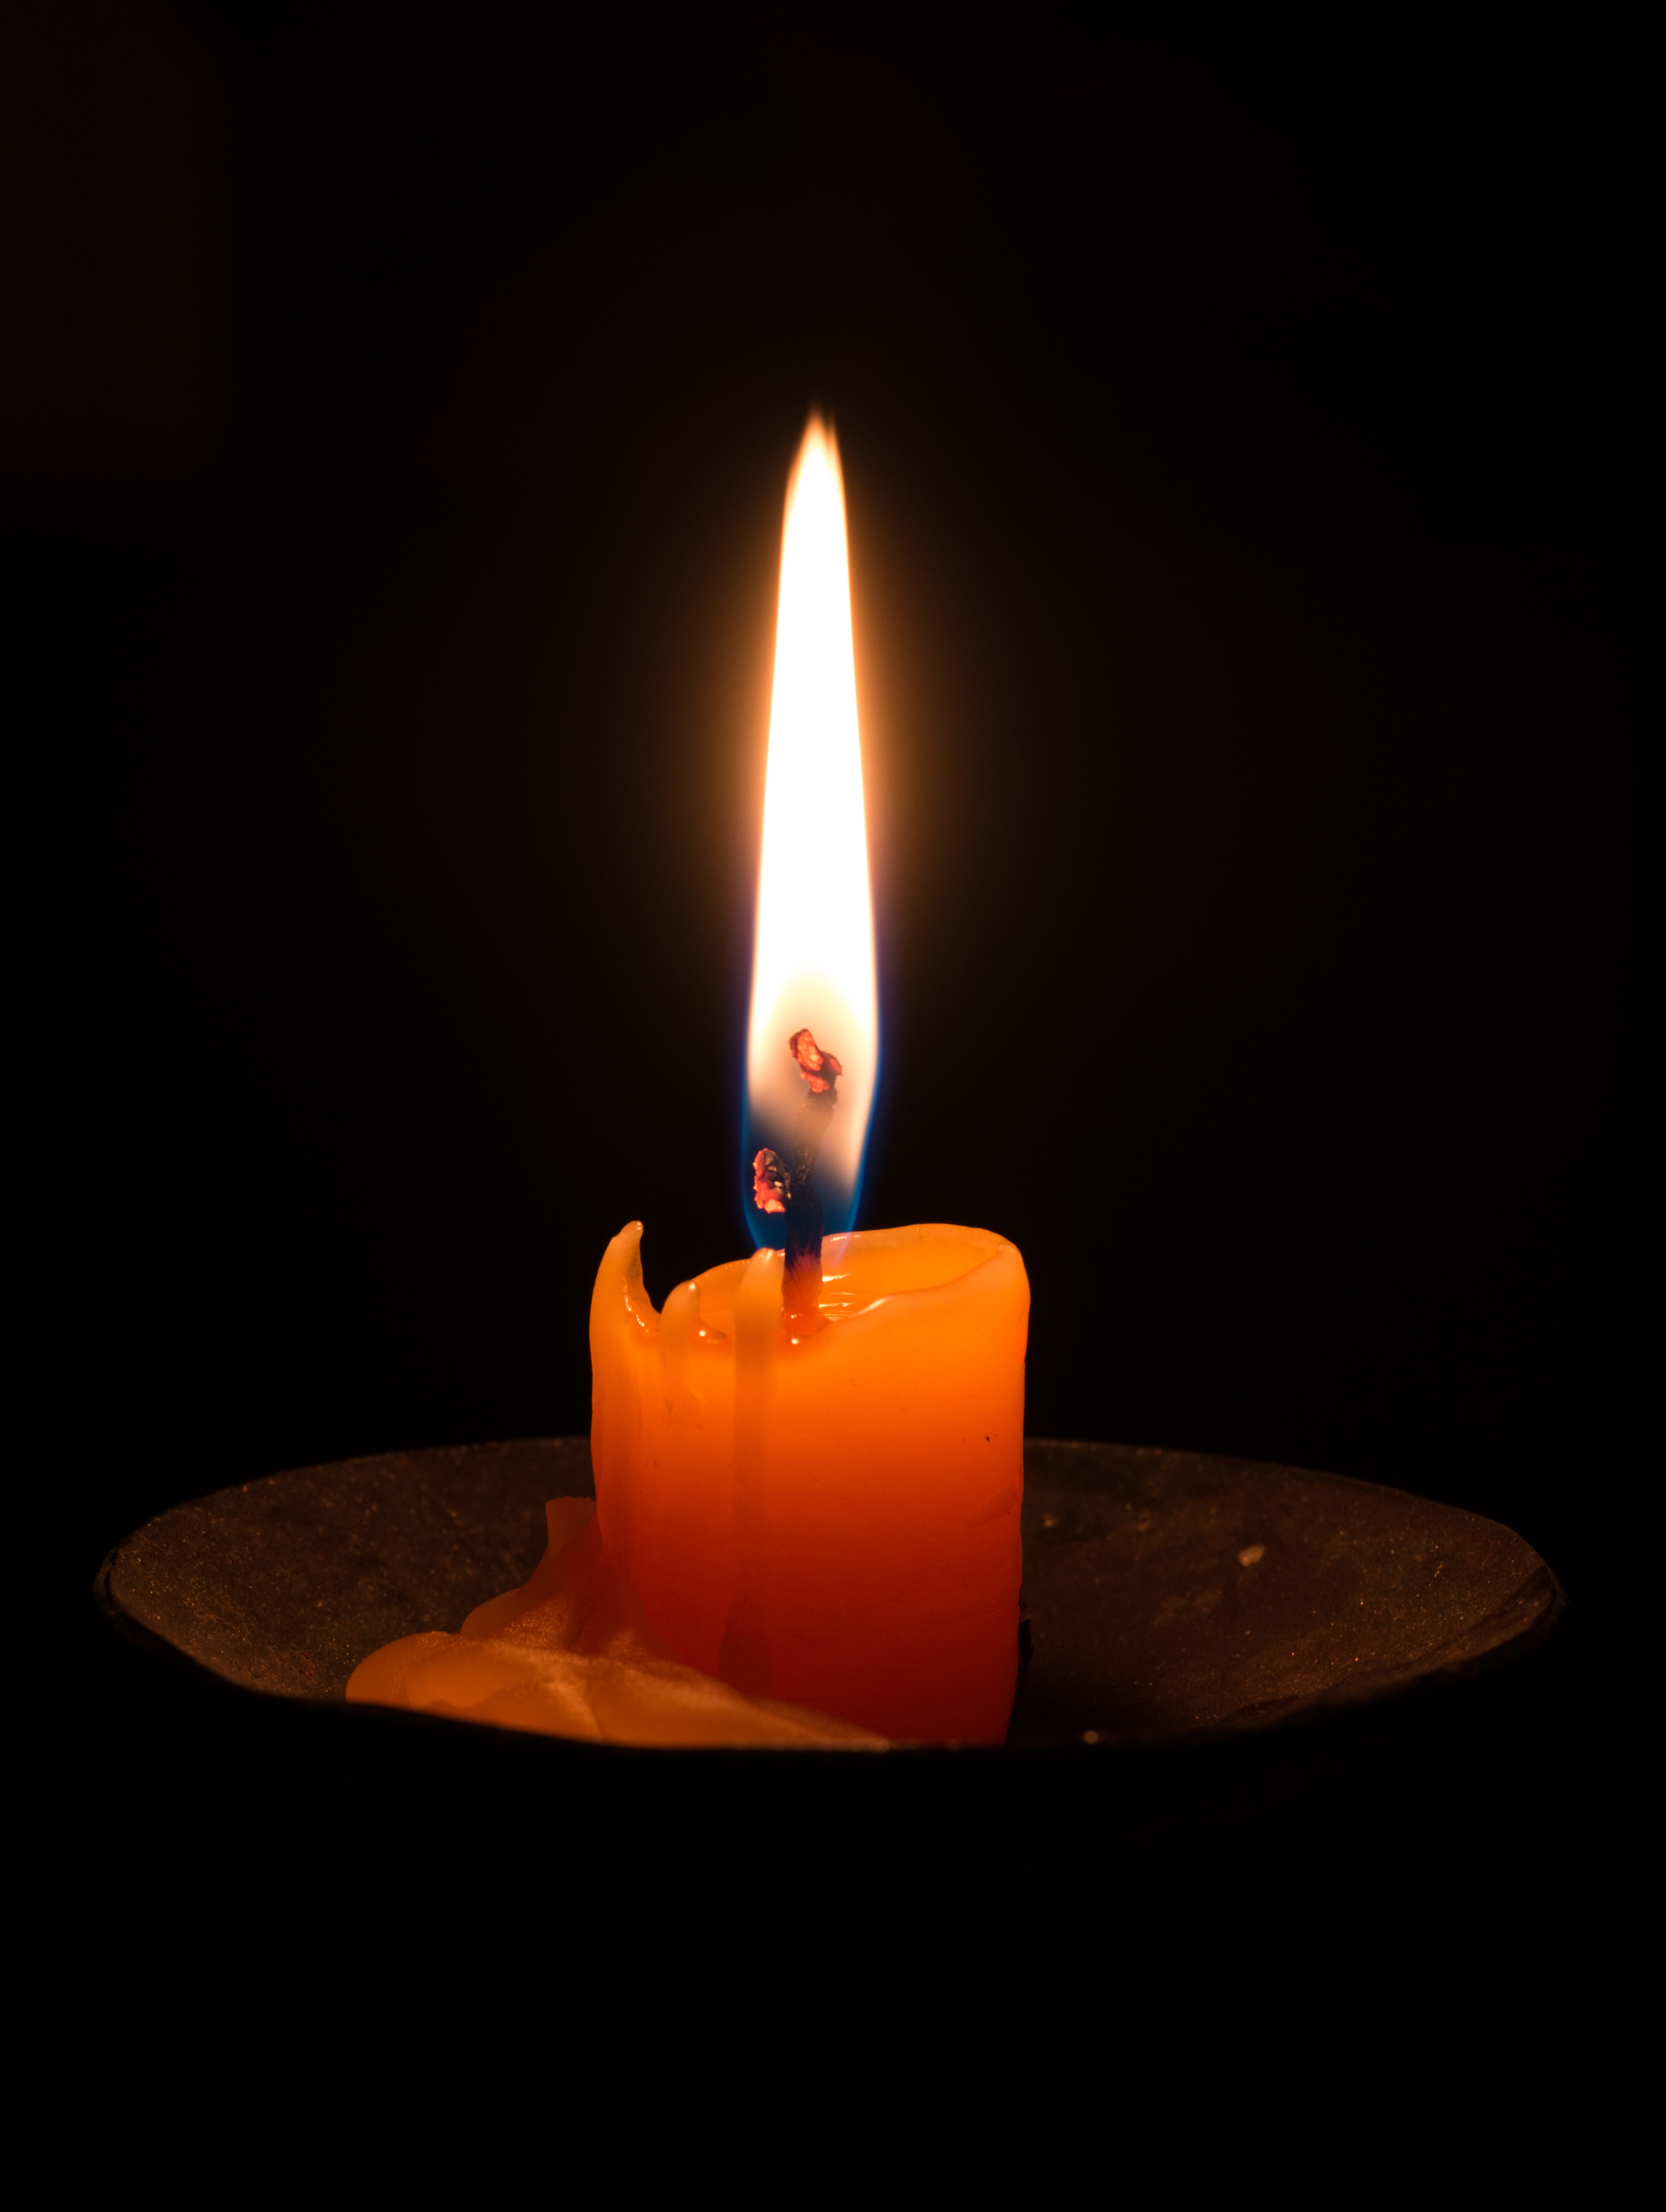
\includegraphics[width=.4\textwidth]{images/L04-candle.jpg}
\end{center}
photo credit: Petar Milošević, Wikimedia Commons, CC-BY-SA 4.0
}

\end{changemargin}
\end{frame}


\begin{frame}
\Large
\begin{changemargin}{1.5cm}
\noindent
Q: What does ``government-granted monopoly'' mean?

\noindent
A: ``The Man'' will come and take you away if you do
not stop the offending behaviour.
\end{changemargin}
\end{frame}


\begin{frame}
\Large
\begin{changemargin}{1.5cm}
\noindent
Q: Which actions are regulated by IP law?

\noindent
A: It depends (on the kind of IP).
\end{changemargin}
\end{frame}

\begin{frame}
\Large
\begin{changemargin}{1.5cm}
\noindent
Q: What kinds of IP are there?

A: The most important kinds of IP for software engineers are:
\vspace*{-2em}
\begin{itemize}
\item copyrights;
\item patents;
\item trade secrets; and
\item trademarks.
\end{itemize}
\end{changemargin}
\end{frame}

\begin{frame}
\frametitle{Your IP}
\Large
\begin{changemargin}{1.5cm}
\vspace*{-2em}
\noindent
At the University of Waterloo, \\
inventors (i.e. you) own\\
the intellectual property they create.

(Though not while you're on co-op).
\end{changemargin}
\end{frame}

\part{About Copyright}
\begin{frame}
\partpage
\vspace*{-12em}\begin{center}\Huge \textcopyright\end{center}
\end{frame}


\begin{frame}
\frametitle{What does copyright do?}
\large
\begin{changemargin}{1cm}
\begin{center}

\includegraphics[width=.2\textwidth]{images/L04-do-not-enter.png}
\\
{\tiny (credit Fry1989, Wikimedia Commons, BY-SA 2.0)}
\end{center}
A copyright owner is allowed to prevent others from:
\vspace*{-1em}
\begin{itemize}
   \item producing and selling copies of the work;
   \item performing/displaying/transmitting the work; and
   \item creating derivative works.
\end{itemize}
\end{changemargin}

\end{frame}


\begin{frame}
\frametitle{What does copyright apply to?}
\Large
\begin{changemargin}{1cm}
Creative works.\\
Examples: code, movies, literary works, maps.

\vspace*{-2em}
Not lists-of-facts,
e.g. phone books.
\end{changemargin}
\end{frame}

\begin{frame}
\frametitle{Who first owns the copyright?}

\begin{changemargin}{1cm}
\Large
\vspace*{-1em}
The author of the work, or for works-for-hire created in the
course of the author's employment, the employer.

Can be sold.
\end{changemargin}
\end{frame}


\begin{frame}
\frametitle{How long does copyright last?}

\begin{changemargin}{1cm}
\Large
\vspace*{-1em}
In Canada, creator's lifetime plus 50 years. \\
In the US, creator's lifetime plus 70 years.
\end{changemargin}
\end{frame}

\begin{frame}
\frametitle{When can you copy?}

\begin{changemargin}{1cm}
\Large
Copyright protections are not absolute; exceptions:
\vspace*{-1em}
\begin{itemize}
\item fair dealing (Canada)/fair use (United States);
\item public domain works;
\item free software/Creative Commons materials.
\end{itemize}
\end{changemargin}
\end{frame}

\begin{frame}
\frametitle{Exceptions to copyright: fair~dealing/fair~use}

\Large
\begin{changemargin}{1cm}
Exceptions to copyright protection, \\
e.g. copying a short excerpt from a book for education is allowed.

(Also, ``classroom exception'': why I can show you videos).

US fair use is more permissive than \\
Canadian fair dealing.

\end{changemargin}
\end{frame}

\begin{frame}
\frametitle{Works not copyrighted: the Public Domain}

\Large
\begin{changemargin}{1cm}
Works on which copyright has expired/was waived can be freely used.

(United States Government works are public domain, but not Canadian government works.)

\end{changemargin}
\end{frame}

\begin{frame}
\frametitle{Copyleft: Free software/Creative Commons}

\Large
\begin{changemargin}{1cm}
Hack the copyright system to allow re-use.

Work is still under copyright, but author grants permission to copy under certain conditions, e.g. must-attribute-author, or (GPL) use only in other GPL'd code.

(Some Open Educational Resources textbooks are coming out which help reduce textbook costs by being freely distributable.)
\end{changemargin}
\end{frame}

\begin{frame}
\frametitle{Sidebar: Plagiarism}
\Large
\begin{changemargin}{1cm}
Plagiarism: not quite the same as copyright infringement.

\vspace*{1em}
\begin{quote}
\emph{Plagiarism is the use of materials for academic credit without permission.}
\end{quote}
\end{changemargin}
\end{frame}

\begin{frame}
\frametitle{Consequences of Plagiarism}
\Large
\begin{changemargin}{1cm}

What happens if caught:
\begin{itemize}
\item meeting with the instructor;
\item typical penalty = 0 on the assignment and -5\% on the course;
\item document case to punish subsequent offenses more severely.
\end{itemize}
\end{changemargin}
\end{frame}

\begin{frame}
\frametitle{Plagiarism Exercise: Some Questions}

\Large
\begin{changemargin}{1cm}
\vspace*{-2em}
Why might you be tempted to plagiarize?

What should you do to avoid plagiarism?
\end{changemargin}
\end{frame}

\part{About Patents}
\begin{frame}
\partpage
\end{frame}

\begin{frame}
\frametitle{What do patents apply to?}
\Large
\begin{changemargin}{1cm}
According to Industry Canada\footnote{\tiny \url{https://www.ic.gc.ca/eic/site/cipointernet-internetopic.nsf/eng/h_wr03652.html}}:

\vspace*{1em}
\begin{quote}
Patents cover new and useful inventions (product, composition, machine, process) or any new and useful improvement to an existing invention.
\end{quote}

That is: you share your invention with the world and get a limited-time monopoly on using your invention.
\end{changemargin}
\end{frame}

\begin{frame}
\frametitle{Software Engineering and Patents}
\Large
\begin{changemargin}{1cm}

It's complicated, and varies country-by-country.

Copyright protects particular implementations.

Patents can (sometimes) protect a process that the computer is carrying out.

\end{changemargin}
\end{frame}

\begin{frame}
\frametitle{Patent Trolls}
\Large
\begin{changemargin}{1cm}

\begin{center}

\includegraphics[width=.2\textwidth]{images/L04-troll.png}
\\
{\tiny (credit Ty Semaka for EFF, BY-SA 2.0; actually a copyright troll}
\end{center}
Some companies own patents \\
but don't build things.

Business model:\\
\hspace*{3em} launch patent infringement lawsuits\\
\hspace*{3em} and settle cases for money.

\end{changemargin}
\end{frame}

\part{About Trade Secrets}
\begin{frame}
\partpage
\end{frame}

\begin{frame}
\Large
\begin{changemargin}{1cm}

\begin{center}

\includegraphics[width=.4\textwidth]{images/L04-coca-cola.png}
\end{center}
A trade secret is information that is not disclosed to the world.

Protected from theft (perhaps by a non-disclosure agreement)
but not from reverse engineering.

Unlike patents, trade secrets do not expire.

\end{changemargin}
\end{frame}

\part{About Trademarks (™)}
\begin{frame}
\partpage
\end{frame}

\begin{frame}
\frametitle{What Trademarks Do}
\Large
\vspace*{-2em}
\begin{changemargin}{1cm}
Protect consumers against confusingly-similar names/identities.
\end{changemargin}
\end{frame}


\end{document}

